%%%%%%%%%%%%%%
% SPACE MATHS
%%%%%%%%%%%%%
\section{Putting the economics and space together \label{sec:spacemaths}}

\begin{comment}
Things to get into this section
%===============================


WUD 39	Role of weight. Weberian. Weight-dependency of fuel use, tech. Normalise people's movement to 1? (But then it changes�)

WUD 38	Basic model dynamic of optimising time use: sets up a zero-sum between labour and space. Is that reasonable? Should fit in with keeping time as the model yardstick.

Value density?

Transport intensity?

Discuss more open approach to externalities -

One could come up with a continuous-space 'externality' description that might match that. Essentially, that's what I do with the density function. But it must be noted it's a black-box solution. At any rate, that's describable using the notation I've used to describe a set of agents in range.

In contrast to this sort of 'black box' approach, I need to define external effects in other ways. So:

As I was discussing above, in backyard: external effects of other actors shifting are constant. Actually, now I think of it, I can point out the slight of hand I'm using - keeping external effects present for any actor until the next time they make a decision.

Anyway: there's an indirect external effect on productivity that will change things, possibly changing actual discrete choices and at least changing output benefits.

There's also a 'black box' external effect imposed based on density. Cf. regional 'externality'�


\end{comment}
%===============================

Having described the essential features going into the thesis models, the job of this section is to explain exactly how those features have been used in model-building. The job of the models themselves is to show what difference particular assumptions about space and agents make for outcomes. What this means for the upcoming section is that definitions are quite open. For example, firms may have a variable number of direct space costs, and people may incur `movement' or `commute' costs - or, as in the core model, neither - depending on what a particular model is examining. Definitions will accordingly be left as open as possible. When it comes to the models themselves, it will be made clear what exact structure is being used.

Section \ref{sec:spaceyspacey} outlined the four types of space used. Regardless of the space-type, actors will face costs stemming from the raw distance involved. Those costs will be defined differently depending on what issue is being examined. For example, people may want to actually move their location and this may incur a cost. Firms moving goods may face a cost for doing so. Equally - as in the core model, where labour and firm migration are both costless - certain space costs may be left out in any particular model. There will, however, be a consistent way of describing what is happening. This is outlined next.
\cmt{Need to outline the structure of this section here.}

\subsection{Types of utility and production function used \label{sec:modelutility_prod}}

Before getting on to describing space, this section briefly explains how utility and production are structured in the models. For the most part, they do not deviate from the simple functions described in section \ref{sec:econconceptsintro}. Both utility and production functions are `black boxes', with a many-to-one input-output structure. \cmt{Functions: may be other, non-black-box versions. Need to check here.}

For production functions, a central requirement is the option to exhibit economies of scale: output per unit of input time must be able to increase as total time goes up. As discussed in section \ref{sec:keyconcepts_coremodel}, the \gls{coremodel} achieves this in a very simple way, with a straight line: $l = a + bx$, where $l$ is the total labour requirement and $a$ and $b$ are the fixed and marginal labour requirement respectively. However, there are some issues when using this in an agent-based context. A full discussion of these can be found in section \ref{sec:agenttimings}; briefly, the fixed labour requirement presents an obstacle to actors `bootstrapping' a model run, and defining firm outcomes in terms of an abstract `total labour requirement' is problematic.

To circumvent these problems, a second form of function capable of economies of scale is used. This production function must meet two needs: to be capable of defining a smooth transition from backyard production, and offer a way to avoid a fixed labour requirement. Backyard production is defined for a single actor only: input of time is directly turned into output of goods linearly for that actor; this linear output makes `space impossible' and actors never have the incentive to move or collaborate. Increasing returns come into play where time input is more than one day in total. 

This is rather tendentious: it has been set up to make non-backyard production always more productive. All that needs to happen to achieve this is a small increase in productivity per unit of input time, compared to backyard production. In-keeping with Krugman's attempts to keep things as simple as possible, there is a straightforward way of achieving this that avoids the need for a minimum time `fixed cost': add a small increment to linear production as time input increases, such that the second derivative of the function is positive. For example, if a small increase in output per unit of time is required -

\[
\frac{dx}{dt}=\frac{t}{10}\]

So -

\[
\intop\frac{t}{10}dt=x=\frac{t^{2}}{20}+C\]

Just add this to linear output to get -

\[
x=t+\frac{t^{2}}{20}+C\]

This gives a simple smooth curve increasing output per unit of time input as time goes up (see figure \ref{fig:backyardtoecons}). A smooth transition from backyard production can then be defined using $C$.

\begin{figure}%
\centering
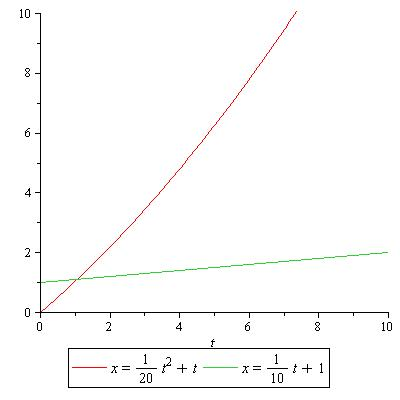
\includegraphics[width=0.5\columnwidth]{ChapterEcon/figures/smoothincretsjpeg}%
\caption{Basic `smooth increasing returns' function, showing total and marginal output.}%
\label{fig:backyardtoecons}%
\end{figure}

Peoples' utility in the models comes from raw good consumption: no price enters directly into their utility function, only good amounts a person can acquire. It is the job of the person to optimise their time to get the best mix of goods they can. In fact (as with the simple production function above) there are difficulties with using optimised utility functions that include price in an agent context: using `raw' good amounts is the best way of letting people find their optima. Again, this is explained in depth in section \ref{sec:twogoodsmodels}. 

%Cut out `space into utility and production', moved to framework.


